\documentclass[10pt,aspectratio=169]{beamer} 
\mode<presentation>{}
%\usepackage{fontspec} %for XeLaTex
\usepackage[T1]{fontenc} 
\usepackage[utf8]{inputenc} 
\usepackage{lmodern}
\usepackage{verbatim}
%\usepackage[danish]{babel} 
\usepackage{amssymb}% http://ctan.org/pkg/amssymb
\usepackage{pifont}% http://ctan.org/pkg/pifont
\usepackage{array}
\usepackage{multirow}
\usepackage{multicol}
\usepackage{graphicx,adjustbox}
\usepackage{booktabs}
\usepackage{dcolumn}
\usepackage{tabulary}
\usepackage{varwidth}
\newcolumntype{P}[1]{>{\raggedright\arraybackslash}p{#1}}
\usepackage{pdfpages}
\usepackage{subcaption}
\usepackage{natbib}
\usepackage{soul}
\usepackage{color,colortbl} %for highlighting table rows
\usepackage[font=scriptsize,labelformat=empty]{caption}
\usepackage{xhfill}% http://ctan.org/pkg/xhfill

\usepackage{tikz} \usetikzlibrary{snakes}
\usepackage{epstopdf}

\usetheme[compress]{Ilmenau} 
\usecolortheme{beaver}
\setbeamercolor*{palette primary}{use=structure,fg=white,bg=gray!60}

\definecolor{beaverred}{RGB}{89,21,26}
\definecolor{beaverred}{RGB}{84,21,18}
\definecolor{bulletblue}{RGB}{30,50,90}
\definecolor{lightbulletblue}{RGB}{130,150,190}
\setbeamercolor{institute in head/foot}{fg=beaverred}
\setbeamercolor{author in head/foot}{fg=beaverred}
\setbeamercolor{section in head/foot}{fg=beaverred,bg=gray!20}
\setbeamercolor{subsection in head/foot}{fg=beaverred,bg=gray!10}
\setbeamercolor{title}{fg=black,bg=white}
\setbeamercolor{item}{fg=bulletblue}
\setbeamercolor{block title}{bg=bulletblue}
\setbeamercolor{itemize item}{fg=lightbulletblue}
\setbeamercolor{itemize subitem}{fg=lightbulletblue}
\setbeamercolor{button}{bg=lightbulletblue,fg=white}

\setbeamertemplate{navigation symbols}{}
\setbeamertemplate{section in toc}{{\color{lightbulletblue}\inserttocsectionnumber} ~\inserttocsection}
\setbeamertemplate{enumerate items}[circle]
\setbeamertemplate{itemize items}[circle]
\setbeamertemplate{subsection in toc}
{\leavevmode\leftskip=2em$\bullet$\hskip1em\inserttocsubsection\par}
\setbeamertemplate{blocks}[rounded][shadow=false] 
\makeatletter
\pgfdeclareverticalshading[lower.bg,upper.bg]{bmb@transition}{200cm}{%
	color(0pt)=(lower.bg); color(2pt)=(lower.bg); color(4pt)=(lower.bg)}

\makeatother
\setbeamerfont{title}{size=\Large}

\setbeamercovered{transparent} %transparent overlays

\title[Municipal Responsiveness]{Responsiveness in Municipal Government}
\author[Egerod \& Larsen]{Benjamin Egerod \qquad Martin Vin\ae s Larsen  \\Department of Political Science \\ University of Copenhagen }
\date[October 30, 2017]{New Avenues In The Study Of Policy	Responsiveness\\ October 30, 2017}

\AtBeginSection[]
{\begin{frame}<beamer>
	\tableofcontents[currentsection,subsectionstyle=show/shaded/hide]
\end{frame}}
\AtBeginSubsection[]
{\begin{frame}<beamer>
\tableofcontents[currentsection,currentsubsection,subsectionstyle=show/shaded/hide]
\end{frame}}

\begin{document}
	
\begin{frame}
\titlepage
\end{frame}

\begin{frame}
\tableofcontents[pausesections,hideallsubsections] %this can be useful if ToC is too long
\end{frame}

\section{Motivation}

\begin{frame}

In most developed countries municipal governments are an essential cog in the machinery of representative government.

\vspace{0.2in} \pause

Yet we know little about the extent to which municipal governments are democratically responsive to the views of their citizens.

\vspace{0.2in} \pause

Some indirect evidence \citep{blom2006parties,folke2014shades,burnett2017politics}, but only a few studies examine it directly \citep{tausanovitch2014representation,einstein2016pushing,sances2017voters}


\vspace{0.2in} \pause

But these are all in the US and either have good measures or a good design.

$\rightarrow$ Our study is in Denmark (for sure) and has both good measures and a good design (hopefully).
\end{frame}

\section[Measure of Municipal Fiscal Policy Conservatism]{An Annual Measure of Municipal Fiscal Policy Conservatism}

\begin{frame}

We collect 14 items on fiscal policy and run them through the following measurement model:


\vspace{0.2in}

\begin{gather*}
F_{itk} \sim N(F^*_{itk}, \phi)\\
F^*_{itk} = \beta_k C_{it} - \alpha_{tk}
\end{gather*}

\vspace{0.2in}

A Bayesian Latent Variable Model.

\end{frame}


\begin{frame}
\begin{table}[h]
	\centering \footnotesize
	%\caption{Indicators of Fiscal Policy Conservatism}
	\label{tab:policies} 
	\begin{tabular}{p{5.5cm}P{3cm}P{4.5cm}} \hline
		\textbf{Policy}                          & \textbf{Availabiliy \newline (number of years)} & \textbf{Do Higher or Lower Values Imply Conservatism?} \\
		\hline
	 \textit{Tax policy} &&\\
		Income tax (pct.)                        & 29     &    Lower       \\
		Property tax (per mille)                      & 29    &    Lower        \\
		Commercial real estate tax (per mille) & 14    &    Lower               \\ \hline
	
	 \textit{Spending policy}  &&\\
		Spending pr. capita (DKK)                & 29    &    Lower        \\
		Spending pr. pupil in school (DKK)       & 7     &    Lower     \\ \hline
		
	\textit{Organization of public service delivery}  &&\\
 		Public Employees (pr. 1,000 citizens)	 & 9	  &	   Lower	     \\
 		Privately operated services  (pct.) &   14  &    Higher     \\
 		Purchases with a private supplier  (pct.)      & 14    &    Higher     \\ \hline
 	
 	 \textit{Co-payment for public services} &&\\   
		Average cost of day care (DKK)                  & 16    &    Higher     \\
		Price of relief stay (DKK)				 & 7	  &	   Higher	 \\
		Food delivery for the  elderly (DKK) & 7   &    Higher     \\
		Stay in nursing home (DKK)              & 7     &    Higher     \\ \hline
	
	 \textit{Extent of Public Services} &&\\ 
		Public housing (pct.)                    & 14     &    Lower               \\
		Class size in public schools	         & 14    &    Lower       \\
		\hline \hline
		\end{tabular}
\end{table} 
\end{frame}

\begin{frame}
	\includegraphics[width=1\textwidth]{images/newtimes_lines.eps}
\end{frame}

\begin{frame}
	\includegraphics[width=1\textwidth]{images/newJoyPlotFiscal.eps}
\end{frame}

\begin{frame}			

The measure has good face validity.

\vspace{0.2in}

Most Conservative muni's: Hørsholm, Gentofte \& Solrød.

\vspace{0.2in}

Most Liberal/Social Democratic: Nakskov, Aarhus \& Odense.

\end{frame}

\section{Local Policy Preferences}

\begin{frame}
We use election results from municipalities to measure local policy preferences.

\vspace{0.2in}
Common in the literature, but not necessarily the ideal.

\vspace{0.2in}
In future iterations: Multi-level Regression with Post-stratification using the DNES.
\end{frame}

\begin{frame}
\begin{figure}
	\begin{subfigure}{0.45\textwidth}
		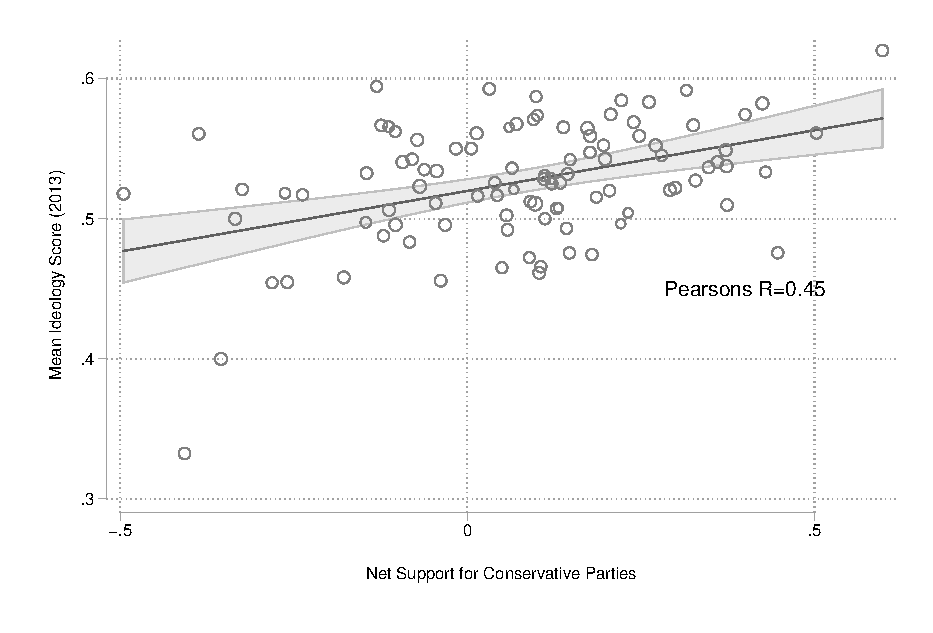
\includegraphics[width=1\textwidth]{images/validation.eps}
		\caption{Does the electorates preference over parties reflect preferences over policy? Data from the 2013 municipal election.} \label{validation1}
	\end{subfigure}  \hfill
	\begin{subfigure}{0.45\textwidth}
		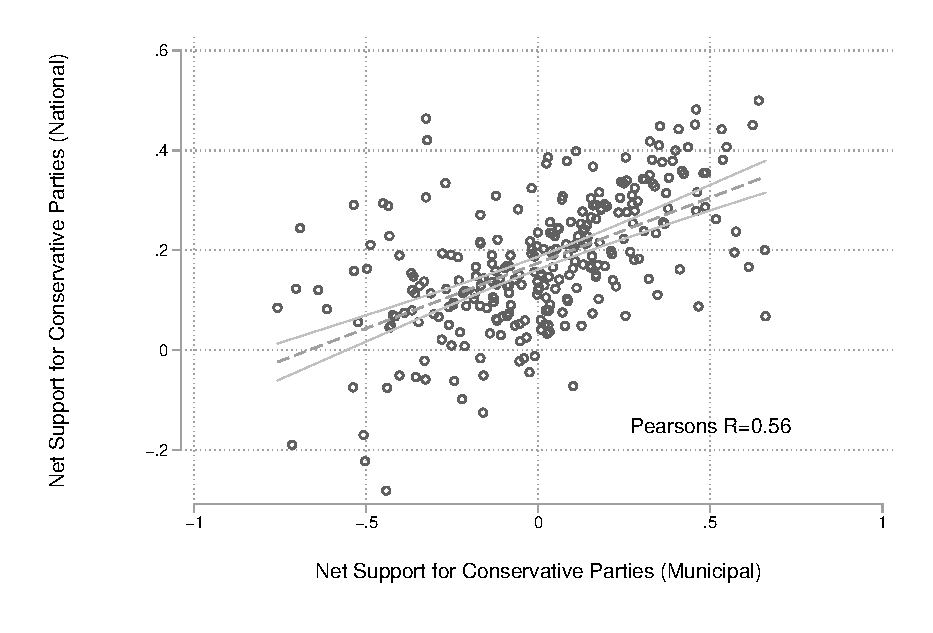
\includegraphics[width=1\textwidth]{images/validation2.eps}
		\caption{How strongly correlated are the electorate's preferences at municipal and national elections? Data from the 2005 municipal and national elections.} \label{validation2}
	\end{subfigure}
\end{figure}
\end{frame}

\begin{frame}
\centering
	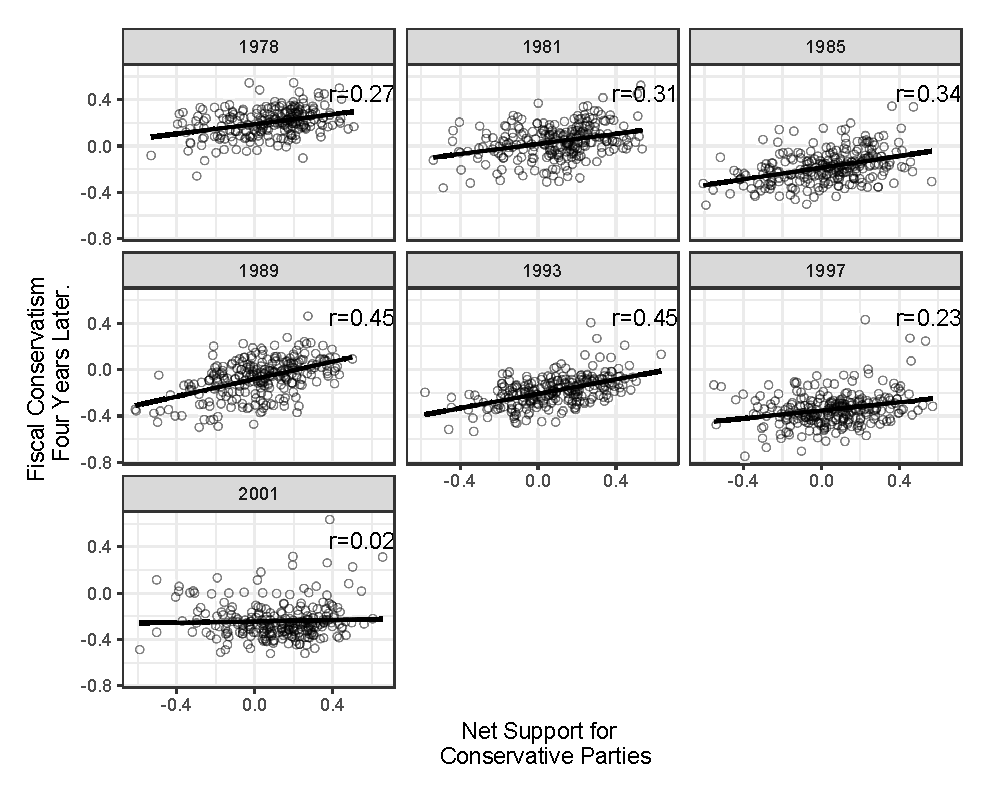
\includegraphics[width=0.7\textwidth]{images/correlations_across_time.eps}
\end{frame}
	
\section[Responsiveness]{Are the Municipalities Responsive?}


\begin{frame}
To estimate responsiveness we use the following model ($\beta$):

\vspace{0.2in}

\begin{equation*}
C_{it+1} =  \beta  V_{it} + \gamma_i +  \pi_t + \theta POP_{it}  +\epsilon_{it},
\end{equation*}

\vspace{0.2in}

A generalized difference in difference model. We may need more controls, but which?

\end{frame}

\begin{frame}	
\begin{columns}
	\column{0.5\textwidth}
If net support for right-wing parties increases with 10 percentage points, then policy becomes 0.02 more conservative. 


\vspace{0.2in} \pause

 If Gentofte got the voters from Albertslund, then they would get the fiscal policy of Slagelse. 

\vspace{0.2in}

If Albertslund got the voters from Gentofte, then they would get the fiscal policy of Frederikssund.

	\column{0.5\textwidth}
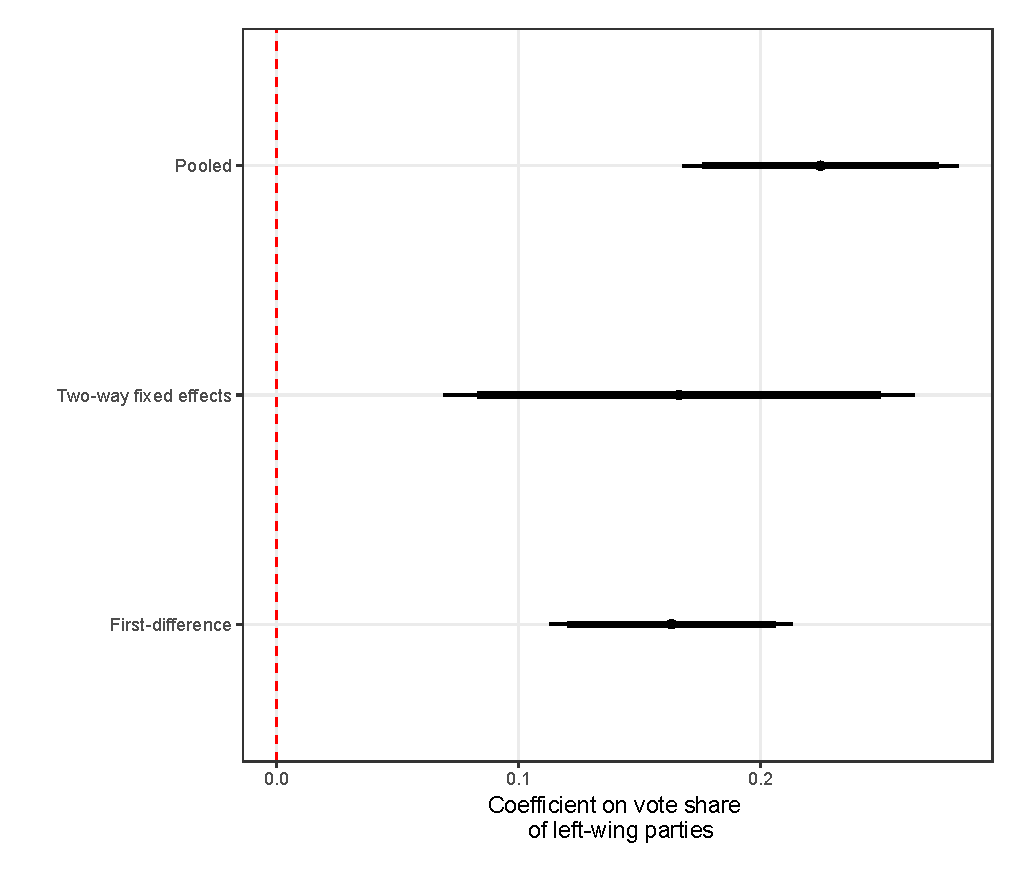
\includegraphics[width=1\textwidth]{images/Newest_ggplot_coef.eps}

\end{columns}
\end{frame}

\begin{frame}			
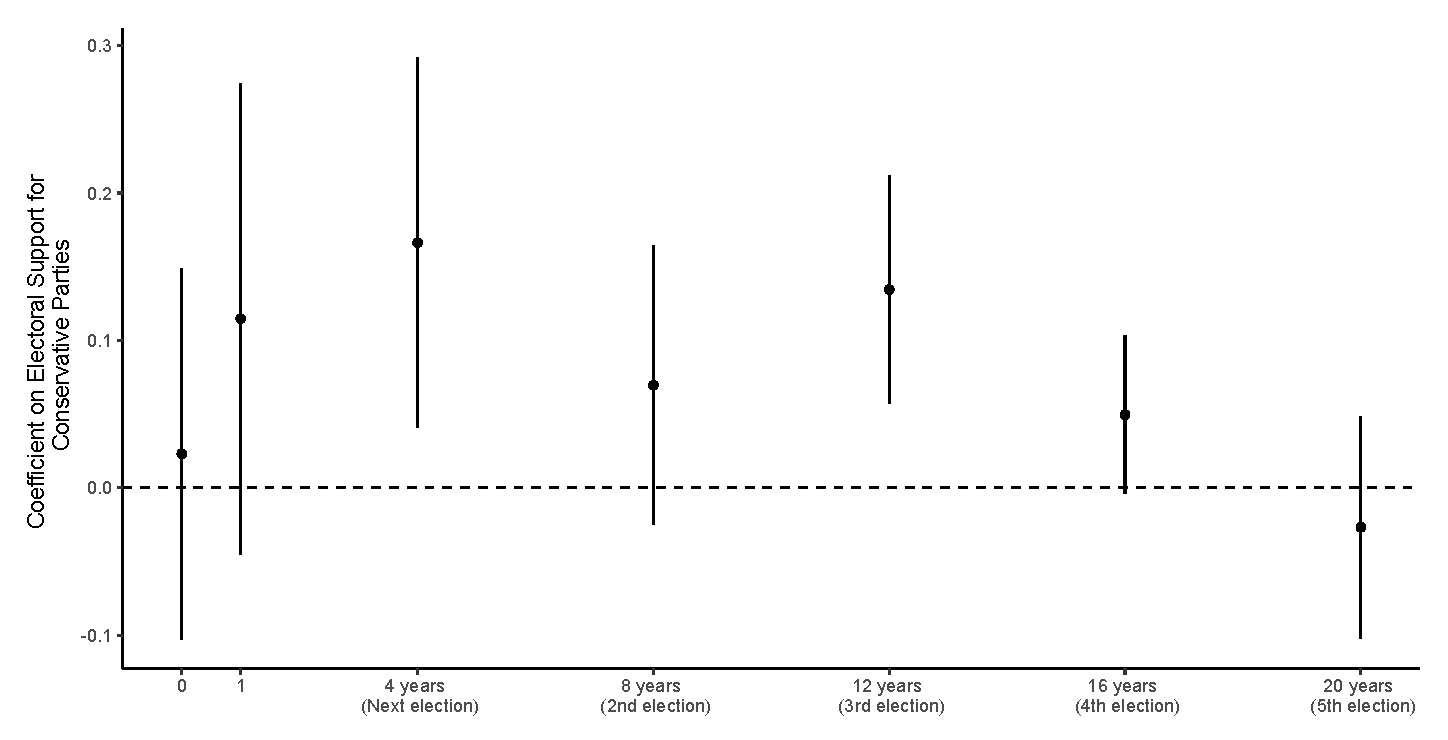
\includegraphics[width=1\textwidth]{images/NoLag_varying_leads.eps}
\end{frame}
	\section[Policy Control]{A Discontinuity in Policy Control}
	
\begin{frame}			
As a final part of our analysis we are interested in examining whether single party majority status affects the level of responsiveness. 

\vspace{0.2in} \pause
Now: Look at deviation between policy preference and policy status quo.

$\rightsquigarrow$ To bring measures on same scale we std and use preference as prior for policy

\vspace{0.2in} \pause

Compare deviation across electoral discontinuity assigning single party majority in city council.

$\rightsquigarrow$ Do councils where largest party narrowly wins/loses majority differ in responsiveness?


\end{frame}

\begin{frame}		
\centering	
	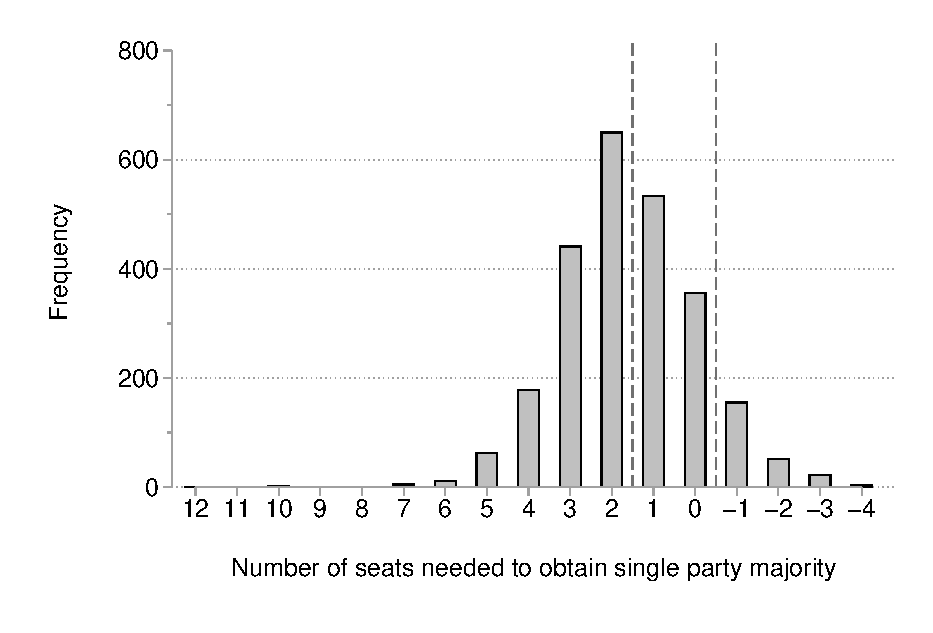
\includegraphics[width=0.8\textwidth]{images/closeelec.eps}
\end{frame}

\begin{frame}
\centering			
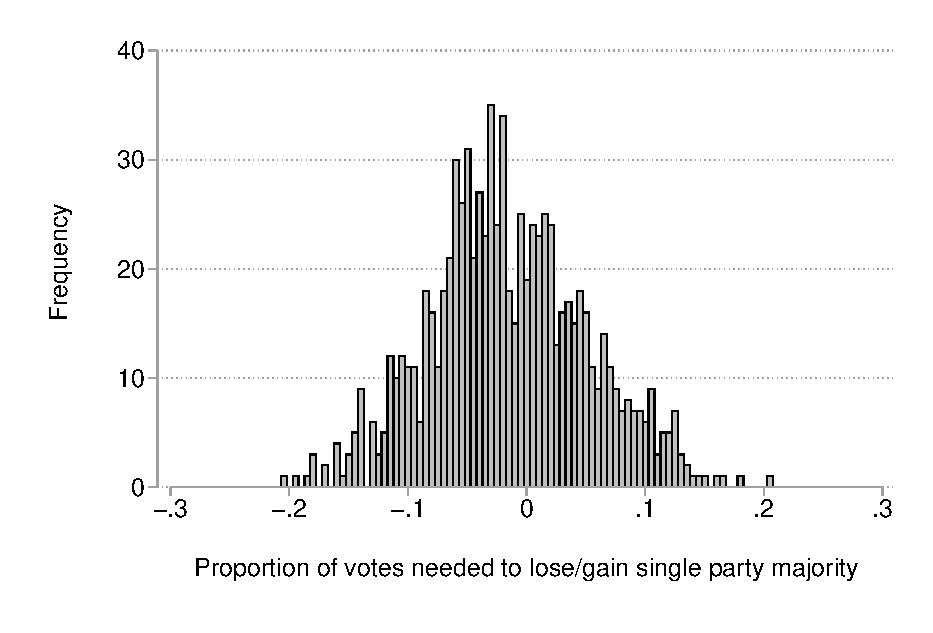
\includegraphics[width=0.8\textwidth]{images/distpct.eps}
\end{frame}

\begin{frame}		
\centering	
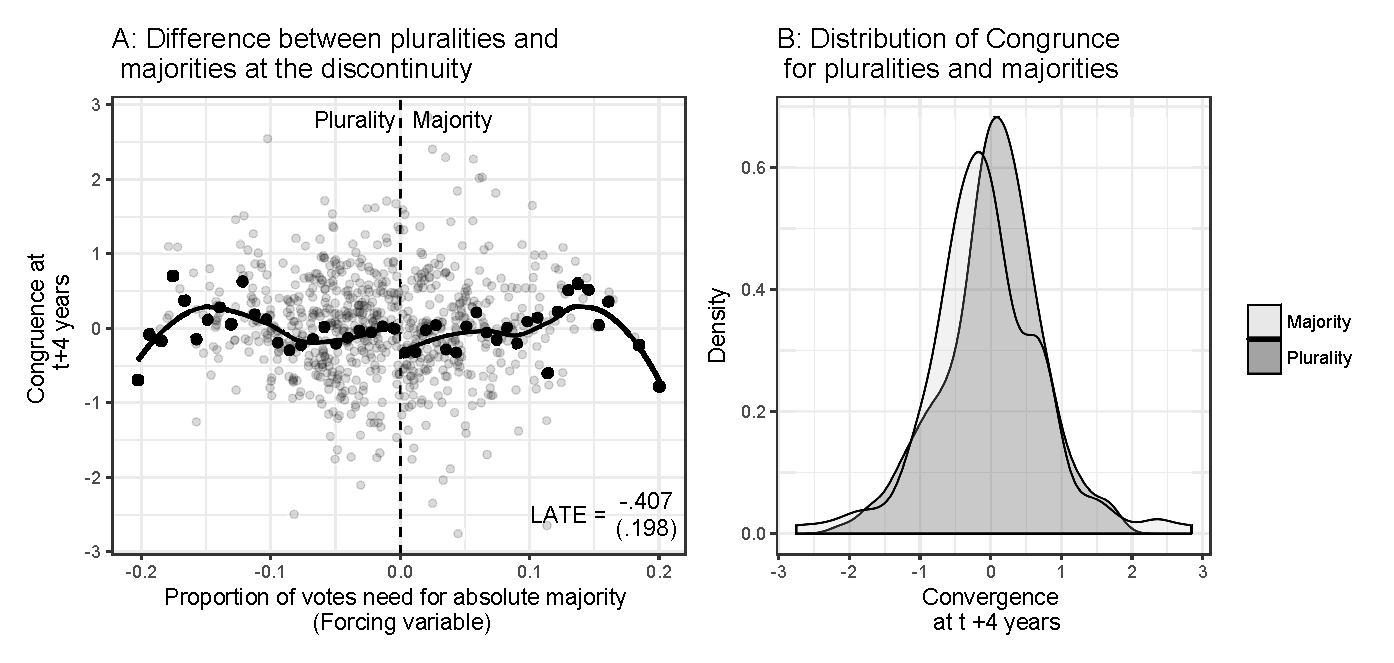
\includegraphics[width=1\textwidth]{images/rddCongruence.eps}
\end{frame}

\begin{frame}	
\centering		
\includegraphics[width=0.5\textwidth]{images/New_robustness_rd3.eps}
\end{frame}

\section[Conclusion]{Where do we go from here?}

\begin{frame}	
This the beginning of a project we hope to extend in various ways. In particular, we are currently pondering some of the following questions.

\begin{enumerate}
	\item Are we missing some important policy items? Is it possible to get better coverage for some of the variables? Is it necessary?
	\item  What controls should we have? They need to have good coverage (span all municipalities across many years).
	\item Should we look at a second country? We might be able to do a scaled down version of this in Norway. 
	\item Should we get a better measure of local policy preferences? We think that we will be able to get municipal level ideological estimates by using MRP to model the left-right question in the Danish National Election Studies.
	\item Should we look more into the general responsiveness analysis or more into the RDD? What is the most interesting?
\end{enumerate}
\end{frame}

\begin{frame}
\bibliographystyle{apa}
\bibliography{bibtex/library}
\end{frame}

\end{document}
	
